\chapter{Objetivos}
Una vez que hemos enfocado el contexto en el que se va a desarrollar este trabajo, pasamos a definir el objetivo general y los sub-objetivos que se pretender cubrir en este TFG.

El objetivo principal es desarrollar, una aplicación web desarrollada con tecnología de última  generación, cuya funcionalidad es facilitar el contacto entre alumnos y profesores para dar clases particulares. Utilizará la geolocalización del alumno para proporcionarle los profesores más próximos a él, además de poder filtrar por diferentes parámetros como curso, asignatura y distancia.

Para la realización de esta aplicación hemos dividido el objetivo general en cuatro sub-objetivos más sencillos con la finalidad de que quitemos complejidad al proyecto.
\begin{enumerate}

    \item Diseño y desarrollo de la parte del cliente es quizás la más tediosa por su dificultad a la hora de desarrollar una interfaz lo suficientemente ligera y adaptable para diferentes tipos de dispositivo. Es por esto que la elección del entorno en el cliente nos puede cambiar por completo la estructura de nuestra aplicación web, además de reducir mucho los tiempos de desarrollo.

    \item Diseño y desarrollo de la parte servidor de la aplicación web, con de la elección de los diferentes entornos que se adaptan mejor a nuestras necesidades. La elección de este entorno viene condicionado en gran medida por el entorno seleccionado para el cliente. Se programará la lógica de la aplicación en el servidor, incluyendo el establecimiento de chat en vivo.

    \item Habrá que diseñar el modelo de datos adecuado para esta aplicación donde los roles de estudiante y alumno aparecen claros. La base de datos por lo general pueden ser de dos tipos SQL y NoSQL, es por esto que debemos elegir cuál de los dos tipos de bases de datos satisface mas con nuestras necesidades.

    \item Una vez que tengamos nuestra aplicación funcionando correctamente en local, habrá que desplegarla en alguno de las plataformas de computación en la nube que ofrecen lo proveedores más importantes como AWS, Azure o GoogleCloud.


\end{enumerate}
\section{Metodología}
En la realización del proyecto se ha seguido una metodología que permite planificar las tareas necesarias para llegar a nuestro objetivo. El modelo seleccionado para la realización del TFG ha sido de tipo cascada, un proceso de desarrollo secuencial, en el que el desarrollo de software se concibe como un conjunto de etapas que se ejecutan una tras otra. Se le denomina así por las posiciones que ocupan las diferentes fases que componen el proyectom colocadas una encima de otra, y siguiendo un flujo de ejecución de arriba hacia abajo, como una cascada.


\begin{figure}[!h]
    \centering
    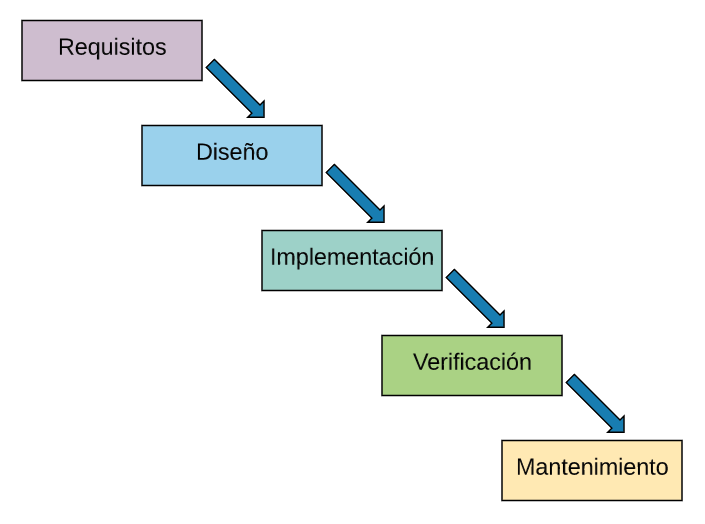
\includegraphics[width=100mm]{img/objetivos/cascada.png}
    \caption{Esquema Metodología Cascada}
\end{figure}

Como parte de la metodología, durante el tiempo que ha durado el proyecto se acordaron reuniones semanales con el tutor de forma presenciales o por Vídeo-Conferencia en las que se revisaban los objetivos semanales y se definían los nuevos hitos. Se ha mantenido también una bitácora describiendo los progresos durante el desarrollo de este TFG \footnote{\url{https://jderobot.org/Graylinx-tfg}}.

También debemos destacar en la metodología el uso de Git como infraestructura de control de versiones de software. El código desarrollado está disponible públicamente en GitHub \footnote{\url{https://github.com/RoboticsURJC-students/2016-tfg-Mario-Fernandez}}. Git es un sistema de control de versiones de código libre y abierto, el cuál esta diseñado para controlar cualquier tipo de proyectos independientemente de su magnitud.

Git mantiene todos los \textit{commit} que hagamos de nuestro proyecto. Un \textit{commit} es una foto de nuestros archivos en un determinado momento. Estos incluyen un identificador, todos los cambios respecto al \textit{commit} anterior y una referencia al mismo. De esta manera, siempre que queramos, podremos retroceder hasta una versión anterior de nuestro código.
Por otro lado, permite tener varias versiones en paralelo o ramas de nuestros proyectos. Éstas son muy útiles para trabajos en equipo, ya que cada desarrollador puede implementar sus funcionalidades en una rama \textit{branch} y luego fusionarse con \textit{(merge)} del resto.

\section{Plan de trabajo}

Para la realización de todo el proyecto se ha seguido un plan de trabajo en cinco diferentes fases:

\begin{itemize}

\item \textbf {Primera fase}: Es una fase de iniciación cuyo objetivo principal es el de aprender todo lo que tenga que ver con el desarrollo web. En esta fase deberíamos dejar conceptos básicos aclarados y empezar a manejar alguna herramienta de control de versiones como Git. Es muy recomendable en esta primera fase empezar a manejar los lenguajes de programación que quieras utilizar en el futuro.

\item \textbf {Segunda fase}: Una vez que tenemos cierta destreza con el desarrollo, empezamos a enfocar nuestra aplicación decidiendo qué tecnologías son las que mejor van a venir para nuestro modelo de aplicación. Esta fase es vital para la continuación del proyecto, ya que la mala elección de una tecnología nos puede llevar mucho tiempo.

\item \textbf {Tercera fase}: Una vez que tenemos claro qué tecnologías vamos a utilizar en nuestra aplicación, comenzamos con un sencillo prototipo que utilice todas las tecnologías que estarán implicadas en nuestra aplicación. Esto nos servirá para tener una sencilla estructura de lo que queremos montar.

\item \textbf {Cuarta fase}: Cuando tengamos claros los conceptos, manejemos los lenguajes de programación necesarios y tengamos montado un sencillo prototipo con las tecnologías que hemos seleccionado para nuestro proyecto, es momento de dar forma a nuestras ideas, extendiendo ese prototipo y aumentando las funcionalidades programadas, es decir desarrollando la aplicación en sí misma.

\item \textbf {Quinta fase}: Cuando tengamos nuestra aplicación completamente desarrollada y haciendo lo que nosotros queremos, es el momento de subirla a alguna plataforma de computación en la nube.
\end{itemize}
